\documentclass[12pt, a4paper]{report}
\usepackage[utf8]{inputenc}
\newcommand\preamble{
    \usepackage[italian]{babel}
    \usepackage{geometry}
    \usepackage{amsmath}
    \usepackage{amssymb}
    \usepackage{graphicx}
    \usepackage{ulem}
    \usepackage[table, dvipsnames]{xcolor}
    \usepackage{spverbatim}
    \usepackage{hyperref}
    \usepackage{pgfplots}

    \pgfplotsset{compat=1.17}

    \geometry{margin=2cm}
    \let\olditemize\itemize
    \renewcommand\itemize{\olditemize\setlength\itemsep{0em}}
    \graphicspath{{Immagini/}}

    \author{Lorenzo Vaccarecci}

    \hypersetup{
        colorlinks=true,
        linkcolor=blue,
        filecolor=magenta,      
        urlcolor=blue,
        pdfpagemode=FullScreen,
    }

    \urlstyle{same}
}
\newcommand {\key}[1]{\underline{#1}}
\newcommand {\question}[1]{\textit{#1}\\}
\newcommand {\important}[1]{\textcolor{red}{#1}}
\newcommand {\remark}[1]{\textcolor{Cyan}{#1}}
\newcommand {\dom}[1]{\text{dom}(#1)}
\newcommand {\img}[1]{\text{img}(#1)}
\newcommand{\inv}[1]{#1^{-1}}
\preamble

\begin{document}
    \begin{titlepage}
        \centering
        \vfill
        {\bfseries\Huge
            Calculus I\\
            \vskip1cm
            \Large
            Lorenzo Vaccarecci\\
            \vskip1cm
            \normalsize
            A.A. 2022/2023
        }
        \vfill
        \vfill
        \vfill
    \end{titlepage}
    \tableofcontents
    \chapter{Nozioni di Base}
    \section{Proprietà di $\mathbb{R}$}
    \begin{enumerate}
        \item \textbf{Densità di $\mathbb{Q} \text{ in } \mathbb{R}$}: $\forall x,y \in \mathbb{R} \quad \exists q \in \mathbb{Q}$ tale che $x<q<y$
        \item \textbf{Densità di $\mathbb{R}-\mathbb{Q} \text{ in } \mathbb{R}$}: $\forall x,y \in \mathbb{R} \quad \exists z \in \mathbb{R}-\mathbb{Q}$ tale che $x<z<y$
        \item Dato $x \in \mathbb{R}$, esiste un \textit{unico} elemento $m \in \mathbb{Z}$ tale che $m \leq x < m+1$. Tale $m$ è detto \textbf{parte intera} di $x$ e si indica con $m=[x]$
    \end{enumerate}
    \section{Grafici}
    L'asse orizzontale è detto \textbf{asse delle ascisse} e quello verticaale \textbf{asse delle ordinate}.
    \begin{itemize}
        \item $(-a,b)$ è simmetrico a $(a,b)$ rispetto all'asse delle ordinate
        \item $(a,-b)$ è simmetrico a $(a,b)$ rispetto all'asse delle ascisse
        \item $(-a,-b)$ è simmetrico a $(a,b)$ rispetto all'origine
        \item $(b,a)$ è simmetrico a $(a,b)$ rispetto alla bisettrice del primo e terzo quadrante
    \end{itemize}
    Traslazione del grafico:
    \begin{itemize}
        \item $f(x)+k$: traslazione verticale verso l'alto
        \item $f(x)-k$: traslazione verticale verso il basso
        \item $f(x+k)$: traslazione orizzontale a sinistra
        \item $f(x-k)$: traslazione orizzontale a destra
    \end{itemize}
    \section{Massimi, minimi, estremi superiori e inferiori}
    \textbf{Definizione}:\\
     Sia $E$ un insieme contenuto in $\mathbb{R}$; $E$ si dice \textbf{limitato superiormente} se esiste un numero molto grande $M$ per cui risulti che $\forall x \in E, x\leq M$. Il numero $M$ si dice \textbf{maggiorante} di $E$.\\
    L'insieme di $E$ si dice \textbf{limitato inferiormente} se esiste un numero molto piccolo $m$ per cui risulti che $\forall x \in E, x\geq m$. Il numero $m$ si dice \textbf{minorante} di $E$.\\
    Se sono verificate entrambe le condizioni ($\forall x \in E, m\leq x \leq M$), allora $E$ si dice \textbf{limitato}.
    \textbf{Esempio:}
    Gli intervalli $(0,1]$ e $(-1,2)$ sono insiemi limitati, mentre $(0,+\infty)$ è limitato inferiormente e $(-\infty,0)$ è limitato superiormente.
    \begin{itemize}
        \item \textbf{Massimo}: Sia $E$ un sottoinsieme non vuoto di $\mathbb{R}$. Diremo che $E$ ammette massimo se $\exists x_{M}\in E \text{ tale che } \forall x \in E, x \leq x_{M}$.  L'elemento $x_{M}$ di $E$ (necessariamente unico) si dice il massimo dell'insieme $E$ e si denota con $\max E$.
        \item \textbf{Minimo}:Sia $E$ un sottoinsieme non vuoto di $\mathbb{R}$. Diremo che $E$ ammette minimo se $\exists x_{m}\in E \text{ tale che } \forall x \in E, x_{m} \leq x$.  L'elemento $x_{m}$ di $E$ (necessariamente unico) si dice il minimo dell'insieme $E$ e si denota con $\min E$.
    \end{itemize}
    \textbf{Esempio:}\\
    L'intervallo $(0,1]$ ha massimo uguale a 1. Non ha minimo. L'intervallo $(-1,2)$ non ha nè massimo nè minimo e l'intervallo $(0,+\infty)$ non ha minimo e $(-\infty,1)$ non ha massimo.\\
    \textbf{Definizione:}\\
    Sia $E$ un sottoinsieme non vuoto e superiormente limitato di $\mathbb{R}$. Il minimo dell'insieme dei maggiornati di $E$ si chiama \textbf{estremo superiore} di $E$ e si denota con $\sup E$.\\
    Sia $E$ un sottoinsieme non vuoto e inferiormente limitato di $\mathbb{R}$. Il massimo dell'insieme dei minoranti di $E$ si chiama \textbf{estremo inferiore} di $E$ e si denota con $\inf E$. Se gli estremi esistono sono \textbf{unici}.
    \begin{itemize}
        \item Un insieme non vuoto e superiormente limitato ha massimo se e solo se il suo estremo superiore appartiene all'insieme.
        \item Un insieme non vuoto e inferiormente limitato ha minimo se e solo se il suo estremo inferiore appartiene all'insieme.
    \end{itemize}
    \textbf{Esempio generale:}\\
    Sia $E=[-1,3)$. L'insieme dei maggioranti di $E$ è $[3,+\infty]$ il minimo di questo insieme è 3. Quindi 3 è l'estremo superiore di $E$ ma non il suo massimo. L'insieme dei minoranti di $E$ è $(-\infty,-1]$ il massimo di questo insieme è -1. Quindi -1 è l'estremo inferiore di $E$ ed è il suo minimo.
    \chapter{Funzioni}
    \begin{equation*}
        f: A \rightarrow B
    \end{equation*}
    \begin{itemize}
        \item $A$ è il dominio di $f$
        \item $B$ è il codominio di $f$
    \end{itemize}
    \section{Iniettività, surgettività, bigettività}
    Una funzione $f: A \rightarrow B$ è detta \textbf{iniettiva} se $\forall x_{1},x_{2} \quad x_{1}\neq x_{2}$ di $A$ risulta che $f(x_{1})\neq f(x_{2})$, ossia se punti distinti hanno immagini distinte. (E' iniettiva se la funzione è continua e solo se è strettamente monotona)\\
    La funzione $f$ è detta \textbf{surgettiva} se $\forall y \in B \quad \exists x \in A | y=f(x)$; ossia ogni elemento del codominio è immagine di qualche punto del dominio.\\
    La funzione $f$ è detta \textbf{bigettiva} se è sia iniettiva che surgettiva.
    \section{Funzioni limitate}
    Una funzione $f$ si dice \textbf{limitata superiormente} se l'immagine è limitata superiormente cioè $\exists M \in \mathbb{R} | \forall x \in A \quad f(x)\leq M$\\
    Una funzione $f$ si dice \textbf{limitata inferiormente} se l'immagine è limitata inferiormente cioè $\exists m \in \mathbb{R} | \forall x \in A \quad f(x)\geq m$\\
    Una funzione $f$ si dice \textbf{limitata} se è sia limitata superiormente che inferiormente cioè $\forall x \in A \quad m\leq f(x)\leq M$.
    \section{Funzioni particolari}
    \subsection{Funzione pari}
    \begin{enumerate}
        \item $f(x)=f(-x) \quad \forall x \in \dom{f}$
        \item Simmetrico rispetto all'asse delle ordinate
    \end{enumerate}
    \subsection{Funzione dispari}
    \begin{enumerate}
        \item $f(x)=-f(-x) \quad \forall x \in \dom{f}$
        \item Simmetrico rispetto all'origine
    \end{enumerate}
    \subsection{Funzione monotòna}
    \begin{itemize}
        \item Descrescente: $\forall x_{1},x_{2} \in \dom{f} \quad x_{1}<x_{2}\rightarrow f(x_{1})\leq f(x_{2})$
        \item Crescente: $\forall x_{1},x_{2} \in \dom{f} \quad x_{1}<x_{2}\rightarrow f(x_{1})\geq f(x_{2})$
    \end{itemize}
    \subsection{Funzione composta}
    \begin{itemize}
        \item $\dom{g\circ f}=\{x\in\dom{f}:f(x)\in \dom{g}\}$ 
    \end{itemize}
    \subsection{Funzione inversa}
    Una funzione $f$ iniettiva è detta invertibile ($\inv{f}$).
    \begin{enumerate}
        \item $\dom{\inv{f}}=\img{f}$
        \item $y=f(x) \iff x = \inv{f}(y)$
        \item $(\inv{f}\circ f)(x)=x \quad \forall x \in \dom{f}$
        \item $(f\circ \inv{f})(y)=y \quad \forall y \in \img{f}$
    \end{enumerate}
    Sia $f$ una funzione strettamente monotòna. Allora $f$ è invertibile e la sua inversa ha la stessa monotonia.
    \subsection{Funzioni elementari}
    \begin{itemize}
        \item $n$ dispari \begin{itemize}
            \item $\sqrt[n]{x^{n}}=x \quad \forall x \in \mathbb{R}$
            \item $(\sqrt[n]{x})^{n}=x \quad \forall x \in \mathbb{R}$
        \end{itemize}
        \item $n$ pari \begin{itemize}
            \item $\sqrt[n]{x^{n}}=|x|  \quad \forall x \in \mathbb{R}$
            \item $(\sqrt[n]{x})^{n}=x \quad \forall x \in [0,+\infty)$ 
        \end{itemize}
    \end{itemize}
    \begin{equation*}
        (a^{m})^{\frac{1}{n}}=\sqrt[n]{a^{m}}
    \end{equation*}
    \subsection{Funzioni esponenziali e logaritmiche}
    \begin{itemize}
        \item Se $a>1$ e $x\in \mathbb{R}$ \begin{equation*}
            a^{x}=\sup\{a^{q}:q\in\mathbb{Q},q\leq x\}
        \end{equation*}
        \item Se $0<a<1$ \begin{equation*}
            a^{x}=\frac{1}{\left(\frac{1}{a}\right)^{x}}
        \end{equation*}
    \end{itemize}
    La funzione esponenziale con base $a\neq 1$ è invertibile perchè è strettamente monotona. La sua inversa è la funzione logaritmica di base $a$ e si indica con $\log_{a}x$.
    \begin{center}
        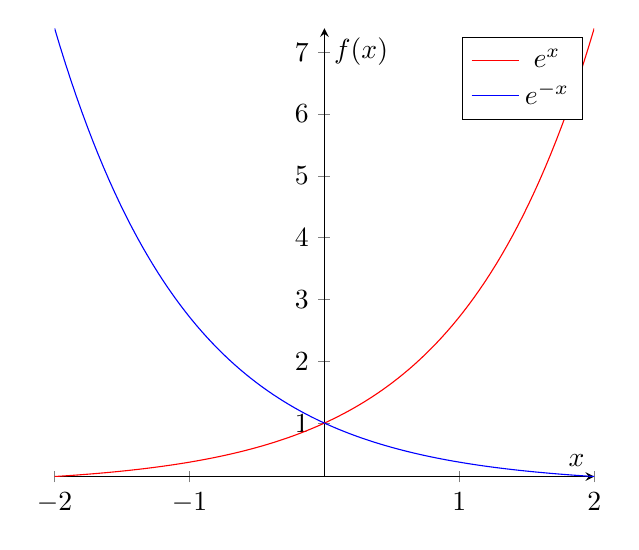
\begin{tikzpicture}
            \begin{axis}[
                axis lines = center,
                xlabel = $x$,
                ylabel = {$f(x)$},
                ytick = {0,1,2,3,4,5,6,7},
            ]
            %Below the red parabola is defined
            \addplot [
                domain=-2:2, 
                samples=100, 
                color=red,
            ]
            {e^x};
            \addplot [
                domain=-2:2, 
                samples=100, 
                color=blue,
            ]
            {e^(-x)};
            \addlegendentry{$e^x$}
            \addlegendentry{$e^{-x}$}
            \end{axis}
        \end{tikzpicture}
    \end{center}
    $e \simeq 2.72$
    \subsection{Funzioni trigonometriche}
    \begin{itemize}
        \item Formule di addizione e sottrazione \begin{itemize}
            \item $\sin(\alpha \pm \beta)=\sin(\alpha)\cos(\beta)\pm \cos(\alpha)\sin(\beta)$
            \item $\cos(\alpha \pm \beta)=\cos(\alpha)\cos(\beta)\pm \sin(\alpha)\sin(\beta)$
        \end{itemize}
        \item Formule di duplicazione \begin{itemize}
            \item $\sin(2x)=2\sin(x)\cos(x)$
            \item $\cos(2x)=2\cos^{2}(x)-1$
        \end{itemize}
        \item $\cos(x+\pi)=-\cos(x)$
        \item $\sin(x+\pi)=-\sin(x)$
        \item $\cos(x+\frac{\pi}{2})=-\sin(x)$
        \item $\sin(x+\frac{\pi}{2})=\cos(x)$
        \item $\tan(x)=\frac{\sin(x)}{\cos(x)}$
    \end{itemize}
    La funzione tangente è dispari e strettamente crescente in ogni intervallo $(-\frac{\pi}{2}+k\pi,\frac{\pi}{2}+k\pi),k\in \mathbb{Z}$
    \chapter{Limiti e continuità}
    \section{Intorno}
    Sia $x_{0}\in \mathbb{R}$ e sia $r>0$ un numero reale. Chiameremo \textbf{intorno di $x_{0}$ di raggio $r$} l'intervallo aperto
    \begin{equation*}
        I_{r}(x_{0})=(x_{0}-r,x_{0}+r)=\{x\in\mathbb{R}:|x-x_{0}|<r\}
    \end{equation*}
    \section{Teorema della permanenza del segno}
    \begin{equation*}
        \lim_{x\to x_{0}}f(x)=l \quad \lim_{x\to x_{0}}g(x)=m 
    \end{equation*}
    Se $l<m$ allora esiste un intorno $I$ tale che $\forall x \in I(x_{0})-x_{0}: f(x)<g(x)$
    \section{Limiti}
    \begin{center}
        \begin{tabular}{|c|c|c|}
            \hline
            $\lim_{x\to x_{0}}f(x)=l$ & &\\
            \hline
            $l\in \mathbb{R}$ & $\forall\varepsilon>0\quad\exists\delta>0\text{ t.c }0<|x-x_{0}|<\delta \text{ e } x\in\dom{f}$ & $|f(x)-l|<\varepsilon$\\
            \hline
            $l=+\infty$ & $\forall M>0\quad\exists\delta>0\text{ t.c }0<|x-x_{0}|<\delta \text{ e } x\in\dom{f}$ & $f(x)>M$\\
            \hline
            $l=-\infty$ & $\forall M>0\quad\exists\delta>0\text{ t.c }0<|x-x_{0}|<\delta \text{ e } x\in\dom{f}$ & $f(x)<-M$\\
            \hline
            $\lim_{x\to +\infty}f(x)=l$ & &\\
            \hline
            $l\in \mathbb{R}$ & $\forall \varepsilon>0\quad\exists b\in\mathbb{R} \text{ t.c. } \forall x>b \text{ e }x\in\dom{f}$ & $|f(x)-l|<\varepsilon$\\
            \hline
            $l=+\infty$ & $\forall M>0\quad\exists b\in\mathbb{R} \text{ t.c. } \forall x>b \text{ e }x\in\dom{f}$ & $f(x)>M$\\
            \hline
            $l=+\infty$ & $\forall M>0\quad\exists N>0\in\mathbb{R} \text{ t.c. } \forall x>N \text{ e }x\in\dom{f}$ & $f(x)>M$\\
            \hline
            $l=-\infty$ & $\forall M>0\quad\exists b\in\mathbb{R} \text{ t.c. } \forall x>b \text{ e }x\in\dom{f}$ & $f(x)<-M$\\
            \hline
            $l=-\infty$ & $\forall M>0\quad\exists N>0\in\mathbb{R} \text{ t.c. } \forall x>N \text{ e }x\in\dom{f}$ & $f(x)<-M$\\
            \hline
            $\lim_{x\to -\infty}f(x)=l$ & &\\
            \hline
            $l\in \mathbb{R}$ & $\forall \varepsilon>0\quad\exists b\in\mathbb{R} \text{ t.c. } \forall x<b \text{ e }x\in\dom{f}$ & $|f(x)-l|<\varepsilon$\\
            \hline
            $l=+\infty$ & $\forall M>0\quad\exists b\in\mathbb{R} \text{ t.c. } \forall x<b \text{ e }x\in\dom{f}$ & $f(x)>M$\\
            \hline
            $l=+\infty$ & $\forall M>0\quad\exists N>0\in\mathbb{R} \text{ t.c. } \forall x<-N \text{ e }x\in\dom{f}$ & $f(x)>M$\\
            \hline
            $l=-\infty$ & $\forall M>0\quad\exists b\in\mathbb{R} \text{ t.c. } \forall x<b \text{ e }x\in\dom{f}$ & $f(x)<-M$\\
            \hline
            $l=-\infty$ & $\forall M>0\quad\exists N>0\in\mathbb{R} \text{ t.c. } \forall x<-N \text{ e }x\in\dom{f}$ & $f(x)<-M$\\
            \hline
        \end{tabular}
    \end{center}
    \begin{itemize}
        \item $\alpha>0$ \begin{itemize}
            \item $\lim_{x\to 0^{+}}x^{\alpha}=0$
            \item $\lim_{x\to +\infty}x^{\alpha}=+\infty$
        \end{itemize}
        \item $a > 1$ \begin{itemize}
            \item $\lim_{x\to +\infty}a^{x}=+\infty$
            \item $\lim_{x\to -\infty}a^{x}=0$
            \item $\lim_{x\to 0^{+}}\log_{a}(x)=-\infty$
            \item $\lim_{x\to +\infty}\log_{a}(x)=+\infty$
        \end{itemize}
        \item $0<a<1$ \begin{itemize}
            \item $\lim_{x\to +\infty}a^{x}=0$
            \item $\lim_{x\to -\infty}a^{x}=+\infty$
            \item $\lim_{x\to 0^{+}}\log_{a}(x)=+\infty$
            \item $\lim_{x\to +\infty}\log_{a}(x)=-\infty$
        \end{itemize}
    \end{itemize}
    \section{Secondo Teorema del confronto (dei carabinieri)}
    \begin{equation*}
        f(x)\leq g(x)\leq h(x) \quad \forall x \in I(x_{0})-\{x_{0}\}
    \end{equation*}
    Se
    \begin{equation*}
        \lim_{x\to x_{0}}f(x)=\lim_{x\to x_{0}}h(x)=l \text{ allora }\lim_{x\to x_{0}}g(x)=l
    \end{equation*}
    \section{Primo Teorema del confronto (caso infinito)}
    \begin{equation*}
        f(x)\leq g(x) \quad \forall x \in I(x_{0})-\{x_{0}\}
    \end{equation*}
    Se 
    \begin{equation*}
        \lim_{x\to x_{0}}f(x)=+\infty \text{ allora }\lim_{x\to x_{0}}g(x)=+\infty
    \end{equation*}
    se
    \begin{equation*}
        \lim_{x\to x_{0}}g(x)=-\infty \text{ allora }\lim_{x\to x_{0}}f(x)=-\infty
    \end{equation*}
    \section{Limite di funzioni monotone}
    \begin{itemize}
        \item Funzione crescente \begin{itemize}
            \item $\lim_{x\to c^{+}}f(x)=\inf\{f(x):x\in I_{+}(c),x>c\}$
            \item $\lim_{x\to c^{-}}f(x)=\sup\{f(x):x\in I_{-}(c),x<c\}$
        \end{itemize}
        \item Funzione decrescente \begin{itemize}
            \item $\lim_{x\to c^{+}}f(x)=\sup\{f(x):x\in I_{+}(c),x>c\}$
            \item $\lim_{x\to c^{-}}f(x)=\inf\{f(x):x\in I_{-}(c),x<c\}$
        \end{itemize}
    \end{itemize}
    \section{Continuità}
    \textbf{Si dice che $f$ è continua in $x_{0}$ se esiste il limite di $f$ in $x_{0}$ ed è uguale a $f(x_{0})$}
    \begin{equation*}
        \lim_{x\to x_{0}}f(x)=f(x_{0})
    \end{equation*}
    Sia $f$ una funzione continua nell'intervallo $I$ allora la sua immagine $f(I)$ è un intervallo.
    \section{Discontinuità}
    \begin{itemize}
        \item \textbf{Di prima specie}:$\lim_{x\to x_{0}}f(x)$ esiste ma $\lim_{x\to x_{0}^{+}}f(x)\neq \lim_{x\to x_{0}^{-}}f(x)$
        \item \textbf{Eliminabile}: $\lim_{x\to x_{0}}f(x)$ esiste ma $\lim_{x\to x_{0}}f(x)\neq f(x_{0})$
    \end{itemize}
    Una funzione può non essere definita in un punto $x_{0}$ ma essere continua in esso, in tal caso si scrive una nuova funzione $f^{*}$:
    \begin{equation*}
        f^{*}(x)=\begin{cases}
            f(x) & x\in \dom{f}\\
            l & x=x_{0}
        \end{cases}
    \end{equation*}
    \section{Continuità della funzione composta}
    \begin{equation*}
        \lim_{x\to x_{0}}f(x)=y_{0}
    \end{equation*}
    \begin{enumerate}
        \item se $y_{0}\in \mathbb{R}$, $g$ è continua in $y_{0}$
        \item se $y_{0}=\pm\infty$, esiste (finito o infinito) $\lim_{y\to y_{0}}g(y)$
    \end{enumerate}
    Allora esiste il limite per $x\to x_{0}$ della funzione composta $g\circ f$ e si ha:
    \begin{equation*}
        \lim_{x\to x_{0}}g(f(x))=g(\lim_{x\to x_{0}}f(x))=\lim_{y\to y_{0}}g(y)
    \end{equation*}
    \section{Teorema degli zeri}
    Sia $f$ una funzione continua su un intervallo chiuso e limitato $[a,b]$. Se $f$ assume valori discordi agli estremi dell'intervallo allora esiste uno zero di $f$ nell'intervallo aperto $(a,b)$.\\
    Siano $f$ e $g$ due funzioni continue in un intervallo chiuso e limitato $[a,b]$ tali che $f(a)<g(a)$ e $f(b)>g(b)$. Allora esiste uno zero nell'intervallo $(a,b)$.
    \section{Valori intermedi}
    Sia $f$ una funzione continua su un intervallo che assume i valori distinti $\alpha$ e $\beta$, allora assume tutti i  valori compresi fra $\alpha$ e $\beta$.
    \section{Del massimo e del minimo o di Weierstrass}
    Sia $f$ una funzione continua nell'intervallo chiuso e limitato $[a,b]$. Allora $f$ assume massimo e minimo.
    \chapter{Derivate}
    \section{Introduzione}
    Coefficiente angolare della retta tangente al grafico nel punto $P$:
    \begin{equation*}
        m_{tan}=\lim_{h\to 0}\frac{f(x_{0}+h)-f(x_{0})}{h}
    \end{equation*}
    Sia $f$ una funzione e siano $x_{0}$ interno al suo dominio e il rapporto $\frac{f(x_{0}+h)-f(x_{0})}{h}$ dove $h$ è detto \textbf{rapporto incrementale}. Si dice che $f$ è derivabile in $x_{0}$ se esiste finito il limite del rapporto incrementale, che si indica con $f'(x_{0})$:
    \begin{equation*}
        f'(x_{0})=\lim_{h\to 0}\frac{f(x_{0}+h)-f(x_{0})}{h}
    \end{equation*}
    Usando il cambiamento di variabile $x=x_{0}+h$ si può riscrivere il limite:
    \begin{equation*}
        f'(x_{0})=\lim_{x\to x_{0}}\frac{f(x)-f(x_{0})}{x-x_{0}}
    \end{equation*}
    Se una funzione $f$ è derivabile in un punto $x_{0}$ allora esiste la retta, non verticale, tangente al grafico di $f$ nel punto $(x_{0},f(x_{0}))$, ed ha equazione:
    \begin{equation*}
        y = f(x_{0})+f'(x_{0})(x-x_{0})
    \end{equation*}
    \begin{itemize}
        \item Se una funzione $f$ è derivabile in un punto $x_{0}$ allora è continua in quel punto.
        %\item Se $f$ non è continua in un punto allora non può essere derivabile in quel punto.
        \item La continuità non implica la derivabilità (viceversa si)
    \end{itemize}
    \section{Derivate destra e sinistra}
    Sia $[x_{0},x_{0}+\delta)\subset \dom{f}$. Si definisce \textbf{derivata destra} di $f$ in $x_{0}$ il limite, se esiste finito:
    \begin{equation*}
        f'_{+}(x_{0})=\lim_{h\to 0^{+}}\frac{f(x_{0}+h)-f(x_{0})}{h}
    \end{equation*}
    Analogalmente si definisce la derivata sinistra che si indica con $f'_{-}(x_{0})$.\\
    Se le derivate destra e sinistra in un punto $x_{0}$ sono (finite e) diverse, allora si dice che in $x_{0}$ la funzione ha un punto angoloso. Osserviamo infine che una funzione è derivabile se e solo se esistono le derivate destra e sinistra e sono uguali.
    \section{Derivata funzione composta}
    \begin{equation*}
        (g\circ f)'(x_{0})=g'(f(x_{0}))\cdot f'(x_{0})
    \end{equation*}
    \section{Massimi e minimi relativi}
    \begin{itemize}
        \item il punto $x_{0}$ è detto \textbf{punto di massimo relativo} se esiste un intorno $I_{\delta}(x_{0})=(x_{0}-\delta, x_{0}+\delta)$ tale che $\forall x \in \dom{f}\cap I_{\delta}(x_{0}) \quad f(x_{0})\geq f(x)$
        \item il punto $x_{0}$ è detto \textbf{punto di minimo relativo} se esiste un intorno $I_{\delta}(x_{0})=(x_{0}-\delta, x_{0}+\delta)$ tale che $\forall x \in \dom{f}\cap I_{\delta}(x_{0}) \quad f(x_{0})\leq f(x)$
    \end{itemize}
    Un punto $x_{0}$ interno al dominio di $f$ si dice un punto critico di $f$ se $f$ è derivabile in $x_{0}$ e $f'(x_{0})=0$.
    \section{Teorema di Fermat}
    Sia $f$ definita in un intorno nel punto $x_{0}$ e derivabile in $x_{0}$. Se $x_{0}$ è un punto di estremo relativo per $f$ allora $f'(x_{0})=0$
    \section{Teorema di Rolle}
    Sia $f$ continua nell'intervallo chiuso e limitato $[a,b]$, derivate nell'intervallo aperto $(a,b)$ e tale che $f(a)=f(b)$. Allora esiste un punto $x_{0}$ nell'intervallo $(a,b)$ t.c. $f'(x_{0})=0$
    \section{Teorema di Lagrange}
    Sia $f$ continua nell'intervallo chiuse e limitato $[a,b]$ e derivabile nell'intervallo aperto $(a,b)$. Allora esiste un punto $x_{0}$ nell'intervallo aperto $(a,b)$ tale che:
    \begin{equation*}
        f(b)-f(a)=f'(x_{0})(b-a)
    \end{equation*}
    \section{Primo teorema di de l'Hôpital}
    Forma indeterminata $\frac{0}{0}$
    \begin{equation*}
        \lim_{x\to x_{0}}\frac{f(x)}{g(x)}=\lim_{x\to x_{0}}\frac{f'(x)}{g'(x)}
    \end{equation*}
    \section{Secondo teorema di de l'Hôpital}
    Forma indeterminata $\frac{\infty}{\infty}$
    \begin{equation*}
        \lim_{x\to x_{0}}\frac{f(x)}{g(x)}=\lim_{x\to x_{0}}\frac{f'(x)}{g'(x)}
    \end{equation*}
    \section{Limite della derivata}
    \begin{equation*}
        \lim_{x\to x_{0}} f'(x)=l \quad \text{allora} \quad \lim_{x\to x_{0}}\frac{f(x)-f(x_{0})}{x-x_{0}}=l
    \end{equation*}
    Segue che se una funzione $f$ è continua in $x_{0}$ ed esiste il limite $\lim_{x\to x_{0}}f'(x)=l$ si ha:
    \begin{itemize}
        \item se $l\in \mathbb{R}$ allora $f$ è derivabile in $x_{0}$ e si ha $f'(x_{0})=l$
        \item se $l=\pm\infty$ allora $f$ non è derivabile in $x_{0}$
    \end{itemize}
    \section{Criterio di monotonia}
    \begin{enumerate}
        \item se $f$ è crescente[decrescente] in $I$ allora $f'(x)\geq 0[f'(x)\leq 0]$ per ogni $x$ in $I$
        \item se $f'(x)\geq 0[f'(x)\leq 0]$ in $I$ allora $f$ è crescente[decrescente] su $I$
        \item se $f'(x)>0[f'(x)<0]$ in $I$ allora $f$ è strettamente crescente[decrescente] su $I$
    \end{enumerate}
    I punti 1 e 2 si possono rovesciare:
    \begin{enumerate}
        \item $f'(x)\geq 0\quad \forall x \in I \iff f$ è crescente su $I$
        \item $f'(x)\leq 0\quad \forall x \in I \iff f$ è decrescente su $I$
    \end{enumerate}
    Mentre non è possibile rovesciare il punto 3.
    \section{Concavità e convessità}
    Sia $f$ una funzione derivabile in $x_{0}$.\\
    Si dice che $f$ è convessa in $x_{0}$ se esiste un intorno $I_{\delta}(x_{0})$ tale che:
    \begin{equation*}
        f(x)\geq f(x_{0})+f'(x_{0})(x-x_{0}) \quad \forall x \in I_{\delta}(x_{0})
    \end{equation*}
    Si diche che $f$ è concava se esiste un intorno $I_{\delta}(x_{0})$ tale che:
    \begin{equation*}
        f(x)\leq f(x_{0})+f'(x_{0})(x-x_{0}) \quad \forall x \in I_{\delta}(x_{0})
    \end{equation*}
    Si diche che $f$ ha un flesso in $x_{0}$ se esiote un intorno $I_{\delta}(x_{0})$ tale che:
    \begin{equation*}
        f(x)\geq f(x_{0})+f'(x_{0})(x-x_{0}) \quad \forall x \in I_{\delta}(x_{0}), x > x_{0}
    \end{equation*}
    \begin{equation*}
        f(x)\leq f(x_{0})+f'(x_{0})(x-x_{0}) \quad \forall x \in I_{\delta}(x_{0}), x < x_{0}
    \end{equation*}
    oppure
    \begin{equation*}
        f(x)\geq f(x_{0})+f'(x_{0})(x-x_{0}) \quad \forall x \in I_{\delta}(x_{0}), x < x_{0}
    \end{equation*}
    \begin{equation*}
        f(x)\leq f(x_{0})+f'(x_{0})(x-x_{0}) \quad \forall x \in I_{\delta}(x_{0}), x > x_{0}
    \end{equation*}
    \chapter{Integrali}
    Sia $f$ una funzione definita sull'intervallo aperto finito o infinito $I$. Una funzione $F:I\to\mathbb{R}$ è detta una primitiva di $f$ in $I$ se è derivabile  in $I$
    \begin{equation*}
        F'(x)=f(x) \quad x\in I
    \end{equation*}
    Ogni funzione continua su un intervallo ammette primitiva.\\
    Sia $f$ una funzione che ammette una primitiva $F$ su un intervallo $I$. Allora la funzione
    \begin{equation*}
        F(x)+c \quad c\in \mathbb{R}
    \end{equation*}
    è una primitiva di $f$ in $I$. Viceversa se $F$ e $G$ sono due primitive di $f$ sull'intervallo $I$ allora esiste una costance $c$ tale che $G(x)-F(x)=c$.\\
    L'insieme di tutte le primitive di $f$ in un intervallo $I$ si chiama \textbf{integrale indefinito} di $f$ sull'intervallo $I$ e si indica con il simbolo:
    \begin{equation*}
        \int f(x)dx
    \end{equation*}
    La funzione $f$ è detta \textbf{funzione integranda}. La variabile $x$ è detta \textbf{variabile di integrazione}.
    \begin{equation*}
        \int f(x)dx=F(x)+c
    \end{equation*}
    \section{Integrale di Riemann}
    Un insieme di punti $\{x_{0},x_{1},\ldots,x_{n}\}$ di intervallo $[a,b]$ tali che $x_{0}=a<x_{1}<\ldots<x_{n}=b$ è detto \textbf{partizione di} $[a,b]$ e verrà denotata con $P(x_{0}\dots x_{n})$ o semplicemente con $P$.\\
    Sia $f$ tale che $m\leq f(x)\leq M$ in $[a,b]$. Date due partizioni $P$ e $Q$ di $[a,b]$ si ha
    \begin{equation*}
        m(b-a)\leq s(f,P)\leq S(f,Q)\leq M(b-a)
    \end{equation*}
    Una funzione $f$ limitata sull'intervallo $[a,b]$ è detta intergabile in $[a,b]$ se esiste un \textbf{unico} numero reale $I$ tale che per ogni partizione $P$ di $[a,b]$ si ha
    \begin{equation*}
        s(f,P)\leq I\leq S(f,P)
    \end{equation*}
    e tale numero è detto \textbf{integrale definito} di $f$ in $[a,b]$ e si indica con il simbolo
    \begin{equation*}
        \int_{a}^{b}f(x)dx
    \end{equation*}
    \subsection{Interpretazione geometrica}
    Se $f\geq 0$ la regione $T$ del piano definita da
    \begin{equation*}
        T=\{(x,y)\in \mathbb{R}^{2}:a\leq x\leq b,0\leq y\leq f(x)\}
    \end{equation*}
    \begin{equation*}
        T = \int_{a}^{b} f(x)dx
    \end{equation*}
    Se $f(x)\leq 0$ in $[a,b]$ si pone
    \begin{equation*}
        T=-\int_{a}^{b}f(x)dx
    \end{equation*}
    Se $f$ non ha segno costante si definisce trapezoide di $f$ su $[a,b]$ la regione $T$ dl piano definita da
    \begin{equation*}
        T=\{(x,y)\in \mathbb{R}^{2}:a\leq x\leq b,0\leq y\leq f(x) \lor f(x)\leq y\leq 0\}
    \end{equation*}
    Sono integrabili sull'intervallo limitato $I$
    \begin{enumerate}
        \item le funzioni limitate in $I$ che hanno al più un numero finito di punti di discontinuità
        \item le funzioni monotone limitate su $I$
    \end{enumerate}
    \section{Teorema della media integrale}
    Sia $f$ una funzione integrabile sull'intervallo $(a,b)$ e siano
    \begin{equation*}
        m=\inf_{x\in (a,b)}f(x) \quad M=\sup_{x\in (a,b)}f(x)
    \end{equation*}
    allora si ha
    \begin{equation*}
        m\leq\frac{1}{b-a}\int_{a}^{b}f(x)dx\leq M
    \end{equation*}
    Se inoltre $f$ è continua in $[a,b]$ allora esiste un punto $c\in (a,b)$ tale che
    \begin{equation*}
        f(c)=\frac{1}{b-a}\int_{a}^{b}f(x)dx
    \end{equation*}
    \section{Teorema fondamentale del calcolo integrale}
    \begin{equation*}
        \forall x \in I \quad F'(x)=f(x)
    \end{equation*}
    Se $f$ è una funzione continua si ha che la \textbf{derivata della sua funzione integrale è $f$}
    \section{Calcolo di aree mediante l'integrale definito}
    Siano $f$ e $g$ due funzioni integrabili sull'intervallo $[a,b]$ e tali che $f(x)\leq g(x)$ per $x\in [a,b]$. Si vuole calcolare l'area della regione $T$ definita da
    \begin{equation*}
        T=\{(x,y):a\leq x\leq b, g(x)\leq y\leq f(x)\}
    \end{equation*}
    \begin{equation*}
        T=\int_{a}^{b} (f(x)-g(x))dx
    \end{equation*}
\end{document}